% !TEX root = MusicFormatsCLIUserGuide.tex

% -------------------------------------------------------------------------
\chapter{Options and help design principles}
% -------------------------------------------------------------------------

\mf\ having many \service s with many options makes options and help handling a challenge.\\
This is why \mf\ provides \oahRepr\ (Options And Help), a full-fledged object-oriented options and help management infrastructure.

\oahRepr\ (Options And Help) is supposed to be pronounced something close to "whaaaah!"
    The intonation is left to the speaker, though...
    And as the saying goes: "\oahRepr? why not!"

OAH organizes the options and the corresponding help in a hierarchy of groups, sub-groups and so-called atoms. OAH is introspective, thus help can be obtained for every group, sub-group or atom at will.

Each pass supplies a OAH group, containing its own options and help. The converters then aggregate the OAH groups of the passes they are composed of to offer their options and help to the user.

\mf\ is equipped with a full-fledged set of options with the corresponding help. Since there are many options and the translation work is done in successive passes, the help is organized in a hierarchy of groups, each containing sub-groups of individual options called \MainIt{atoms}.

The \optionName{query} option used through-out this document will be presented in detail at \sectionRef{Querying about options by name}.


The term {\it \CLI} means that the user launches the \mf\ \service s in a terminal window, using a so-called \MainIt{shell}. A shell writes a so-called \MainIt{prompt} in the window, indicating that is waits for user input at the keyboard, and performs a loop:
\begin{itemize}
\item it \MainIt{reads} a line from the keyboard, made of a command name, options and arguments;
\item the command is analyzed to check that it is \MainIt{well-formed};
\item the command is \MainIt{executed} if it is well-formed;
\item the shell displays the prompt again and waits for the next user input.
\end{itemize}

When a terminal window is created, a shell is launched automatically, waiting for user in put in that window.

Various shell families have been created over time. The most widely used today is \Main{Bash} (\url{https://www.gnu.org/software/bash/}). No worry though, the information presented in this section applies to all of them.


% -------------------------------------------------------------------------
\chapter{Options use}
% -------------------------------------------------------------------------

THe \oahRepr\ options are very easy to use. They are inspired by \Main{GNU} options, with more power and flexibility:
\begin{itemize}
\item the options can be supplied in the \CLI\ as usual;

  \item they can also be supplied in a call to an \API\ \Main{function} such as \functionName{musicxmlfile2lilypond}, in an options and arguments argument. \\
    		See the \docpdf{MusicFormatsAPIUserGuide}{MusicFormatsAPIUserGuide} for the details;

%%%JMI https://github.com/jacques-menu/musicformats/blob/dev/documentation/MusicFormatsAPIUserGuide/MusicFormatsAPIUserGuide.pdf

\item options are introduced either by \code{-} or \code{--}, which can be used at will. Both ways are equivalent;

\item all options have a long name, and some have a complementary short name.
 The latter is not provided if the long name is short enough, such as \optionName{jianpu}, \optionName{cubase}, \optionName{ambitus} or \optionName{custos}.\\
    Short and long names can be used and mixed at will in the \CLI\ and in option vectors (\API).
    Apart from very common options such as \optionName{o}, the short names are meant for interactive use. This document uses only long name, which are more explicit in general;

\item some short option names are supplied as is usual in open sotfware, such as \optionName{h} (help), and \optionName{o} (output file name):
\begin{lstlisting}[language=Terminal]
jacquesmenu@macmini > xml2ly -query o
--- Help for atom "o" in subgroup "Files"
    -output-file-name, -o FILENAME
          Write output to file FILENAME instead of standard output.
\end{lstlisting}

\item options and arguments such as file names can be intermixed at will. Thus:
\begin{lstlisting}[language=Terminal]
xml2ly --display-cpu-usage basic/HelloWorld.xml
\end{lstlisting}
and
\begin{lstlisting}[language=Terminal]
xml2ly basic/HelloWorld.xml -display-cpu-usage
\end{lstlisting}

produce the exact same result;

\item some options names, either long or short, share a common \Main{prefix}. This allows them to be \MainIt{contracted}, as in \code{-h=rests,notes}, which is equivalent to \code{-hrests, -hnotes}, and \code{-trace=voices,notes}, equivalent to \code{-trace-voices, -trace-notes}:
\begin{lstlisting}[language=Terminal]
jacquesmenu@macmini > xml2ly -query h
--- Help for prefix "h" ---
        '-h=abc,wxyz' is equivalent to '-habc, -hwxyz'

--- Help for atom "h" in subgroup "Options and help"
    -help, -h
          Display xml2ly's full help.
\end{lstlisting}

\item the single-character options can be \MainIt{clustered}: \optionName{vac} is equivalent to: \code{-v, -a, -c}:
\begin{lstlisting}[language=Terminal]
jacquesmenu@macmini > xml2ly -va
Command line version of musicxml2lilypond converter v0.9.52 (November 29, 2021)
A member of MusicFormats v0.9.59 (January 4, 2022)

Representations versions:
  MXSR
    v0.9.5 (October 6, 2021)
  MSR
    v0.9.52 (November 27, 2021)
  LPSR
    v0.9.5 (October 6, 2021)

Passes versions:
  mxsr2msr
    v0.9.51 (November 27, 2021)
  msr2msr
    v0.9.51 (November 15, 2021)
  msr2lpsr
    v0.9.5 (October 6, 2021)
  lpsr2lilypond
    v0.9.52 (December 16, 2021)
What xml2ly does:

    This multi-pass converter basically performs 5 passes:
        Pass 1:  reads the contents of MusicXMLFile or stdin ('-')
                 and converts it to a MusicXML tree;
        Pass 2a: converts that MusicXML tree into
                 a first Music Score Representation (MSR) skeleton;
        Pass 2b: populates the first MSR skeleton from the MusicXML tree
                 to get a full MSR;
        Pass 3:  converts the first MSR into a second MSR to apply options
        Pass 4:  converts the second MSR into a
                 LilyPond Score Representation (LPSR);
        Pass 5:  converts the LPSR to LilyPond code
                 and writes it to standard output.

    Other passes are performed according to the options, such as
    displaying views of the internal data or printing a summary of the score.

    The activity log and warning/error messages go to standard error.
\end{lstlisting}

\end{itemize}


% -------------------------------------------------------------------------
\section{Options characteristics}\label{Options characteristics}
% -------------------------------------------------------------------------

There are various options in \mf\ for various needs. Every option controls a feature of a component or specifies a value used in the operation of the library.

An option can be:
\begin{itemize}
\item pure help:
it provides information to the user, but does not do anything musical, such as \optionBoth{contact}{c}:
\begin{lstlisting}[language=Terminal]
jacquesmenu@macmini > xml2ly -contact
To contact the maintainers of xml2ly:
    Create an issue at https://github.com/jacques-menu/musicformats,
    describing the problem and any error messages you get if relevant.
    You should sign up for d GitHub for that.
\end{lstlisting}

\item self-sufficient, such as \optionBoth{quiet}{q}:
\begin{lstlisting}[language=Terminal]
jacquesmenu@macmini > xml2ly -query quiet
--- Help for atom "quiet" in subgroup "Warning and errors"
    -quiet, -q
          Don't issue any warning or error messages.
\end{lstlisting}

\item expecting a value, which must be supplied right after the option name:
\begin{lstlisting}[language=Terminal]
jacquesmenu@macmini > xml2ly -query msr-pitches-language
--- Help for atom "msr-pitches-language" in subgroup "Notes"
    -msr-pitches-language, -mplang LANGUAGE
          Use LANGUAGE to display note pitches in the MSR logs and text views.
          The 13 MSR pitches languages available are:
          arabic, catalan, deutsch, english, espanol, francais,
          italiano, nederlands, norsk, portugues, suomi, svenska and vlaams.
          The default is 'kQTPNederlands'.
\end{lstlisting}

\item expecting an optional value, supplied with a '=' without any spaces:
a default value is used if none is provided by the user, such as \optionNameBoth{name-help}{nh}, presented in more detail at \sectionRef{Querying about options by name}:
\begin{lstlisting}[language=Terminal]
jacquesmenu@macmini > xml2ly -name-help=output-file-name
--- Help for atom "output-file-name" in subgroup "Files"
    -output-file-name, -o FILENAME
          Write output to file FILENAME instead of standard output.
\end{lstlisting}

\end{itemize}

Some options can be used \MainIt{several times}, while the others can be used only once.

% -------------------------------------------------------------------------
\section{The {\tt -insider} option}
% -------------------------------------------------------------------------

As mentioned above, the \mf\ library components, i.e. \representation s, \pass es, \converter s and \generator s, have options and help attached to them. There are also other 'global' sets of options, independently of the individual components themselves.

\mf\ has to 'modes' for options and help handling:
\begin{itemize}
\item in \MainIt{regular} mode, the default, the options are grouped by subject, such as tuplets or chords. In other words, there are grouped in a user-oriented way;
\item in \MainIt{insider} mode, they are grouped as there are used internally by MusicFormats behind the scenes, in an implementation-oriented way, hence the name.
\end{itemize}

Switching from the default regular mode to the insider mode is done with the \optionNameBoth{insider}{ins} option:
\begin{lstlisting}[language=Terminal]
jacquesmenu@macmini > xml2ly -query insider
--- Help for atom "insider" in subgroup "Options and help"
    -insider, -ins
          Use the 'insider' mode for the options and help,
          in which the options are grouped as they are used internally by MusicFormats.
          In the 'regular' defaut mode, they are grouped by user-oriented topics,
          such a slurs, tuplets and figured bass.
\end{lstlisting}

In regular mode, the options are displayed in subgroups only. The groups containing them are not displayed for simplicity, because a three-level options hierarchy is not what users expect and are used to.

For example, the \optionNameBoth{ignore-ornaments}{oorns} option is displayed this way in regular mode:
\begin{lstlisting}[language=Terminal]
jacquesmenu@macmini > xml2ly -query ignore-ornaments
--- Help for atom "ignore-ornaments" in subgroup "Ornaments"
    -ignore-ornaments, -oorns
          Ignore ornaments in MusicXML data.
\end{lstlisting}

In insider mode, on the contrary, the full group-subgroup-atom hierarchy is visible, as well as the attachment of the options to the groups managed internally by \mf:
\begin{lstlisting}[language=Terminal]
jacquesmenu@macmini > xml2ly -query ignore-ornaments -insider
--- Help for atom "ignore-ornaments" in subgroup "Notes" of group "mxsr2msr" ---
    -ignore-ornaments, -oorns
          Ignore ornaments in MusicXML data.
\end{lstlisting}

To summarize things up, it can be said that the regular mode offers a user-oriented \MainIt{view} of the options available in the insider mode.


% -------------------------------------------------------------------------
\section{Early options}
% -------------------------------------------------------------------------

A particular case of options is the \MainIt{early options}, which are taken into account prior to the options being actually analyzed.
This the case of \optionBoth{insider}{ins}, since the whole set of possible options depends on it being used or not.

An \earlyOption\ should be supplied in the \CLI\ itself. Having it in included options and arguments files prevents it from being applied early. See \chapterRef{Including options and arguments from a file} about this feature.


% -------------------------------------------------------------------------
\chapter{Options and help introspection}
% -------------------------------------------------------------------------

% -------------------------------------------------------------------------
\section{Restricting help to a given group or subgroup}
% -------------------------------------------------------------------------

The \oahRepr\ groups and subgroups can be displayed with their own options, such as \optionBoth{help-midi}{hmidi}:
\begin{lstlisting}[language=Terminal]
jacquesmenu@macmini: ~ >  xml2ly -help-midi
--- Help for subgroup "MIDI" in group "MIDI group" ---
  MIDI group (-help-midi-group, -hmidi-group):
  --------------------------
    MIDI (-help-midi, -hmidi):
      -no-midi
            Generate the '\midi' block as a comment instead of active code.
      -midi-tempo, -mdtempo MIDI_TEMPO_SPEC
            Generate a '\tempo' command in the \midi block.
            MIDI_TEMPO_SPEC can be:
            'DURATION = PER_SECOND'
            or
            "DURATION = PER_SECOND" .
            DURATION is a string such as '8.', and PER_SECOND is an integer.
            The single or double quotes are used to allow spaces around the '=' sign,
            otherwise they can be dispensed with.
            Using double quotes allows for shell variables substitutions, as in:
            PER_SECOND=66
            xml2ly -midiTempo "8. ${PER_SECOND}" .
            The default is '8 = 180'.
\end{lstlisting}


% -------------------------------------------------------------------------
\section{Querying about options by name}\label{Querying about options by name}
% -------------------------------------------------------------------------

One can obtain help on any specific group, sub-group or atom with the \optionName{query} option:
\begin{lstlisting}[language=Terminal]
jacquesmenu@macmini > xml2ly -query query
--- Help for atom "query" in subgroup "Options and help"
    -query OPTION_NAME
          Print help about OPTION_NAME.
\end{lstlisting}

\begin{lstlisting}[language=Terminal]
jacquesmenu@macmini > xml2ly -query output-file-name
--- Help for atom "output-file-name" in subgroup "Files"
    -output-file-name, -o FILENAME
          Write output to file FILENAME instead of standard output.
\end{lstlisting}

Another option exists to obtain the same result: \optionNameBoth{name-help}{nh} has an optional value:
\begin{lstlisting}[language=Terminal]
jacquesmenu@macmini > xml2ly -name-help=output-file-name
--- Help for atom "output-file-name" in subgroup "Files"
    -output-file-name, -o FILENAME
          Write output to file FILENAME instead of standard output.
\end{lstlisting}

The default value if none is supplied is\dots \code{name-help} itself:
\begin{lstlisting}[language=Terminal]
jacquesmenu@macmini > xml2ly -name-help
--- Help for atom "name-help" in subgroup "Options and help"
    -name-help, -nh OPTION_NAME
          Print help about OPTION_NAME.
          OPTION_NAME is optional, and the default value is 'name-help'.
\end{lstlisting}

Choosing one option of the other is a matter of taste. To be honest, \optionNameBoth{name-help}{nh} has been created to illustrate optional values\dots


% -------------------------------------------------------------------------
\section{Searching the help for a string}
% -------------------------------------------------------------------------

The \mf\ \service s have a great number of options. \Option{find} comes in handy to search the available help:
\begin{lstlisting}[language=Terminal]
jacquesmenu@macmini > xml2ly -query find
--- Help for atom "find" in subgroup "Options and help"
    -find STRING
          Find string STRING in the help.
          The search is case insensitive, and a '-' is added in front of options names for clarity.
\end{lstlisting}

\begin{lstlisting}[language=Terminal]
jacquesmenu@macmini > xml2ly -find output-file-name
2 occurrences of string "output-file-name" have been found:
   1:
    -output-file-name, -o FILENAME
    Write output to file FILENAME instead of standard output.
   2:
    -auto-output-file-name, -aofn
    This option can only be used when writing to a file.
                    Writethe output to a file in the current working directory.
                    The file name is derived from that of the input file:
                    any suffix after the '.' is replaced by one suited for the output format,
                    or such a suffix is adde if no '.' is present.
\end{lstlisting}


% -------------------------------------------------------------------------
\section{Displaying help about options usage}
% -------------------------------------------------------------------------

A minimal version of this chapter is displayed by the \optionNameBoth{-help-options-usage}{hou} option:
\begin{lstlisting}[language=Terminal]
jacquesmenu@macmini > xml2ly -help-options-usage
xml2ly options usage:
  In xml2ly, '-' as an argument, represents standard input.

  Most options have a short and a long name for commodity.
  The long name may be empty if the short name is explicit enough.

  The options are organized in a group-subgroup-atom hierarchy.
  Help can be obtained for groups or subgroups at will,
  as well as for any option with the '-name-help, -nh' option.

  A subgroup can be showm as a header only, in which case its description is printed
  only when the corresponding short or long names are used.

  Both '-' and '--' can be used to introduce options,
  even though the help facility only shows them with '-'.

  There some prefixes to allow for shortcuts,
  such as '-t=voices,meas' for '-tvoices, -tmeas'.

  The options can be placed in any order,
  provided the values immediately follow the atoms that need them.

  Using options that attempt to create files, such as '-o, -output-file-name',
  leads to an error if the environment is read-only access,
  as is the case of https://libmusicxml.grame.fr .
\end{lstlisting}


% -------------------------------------------------------------------------
\section{Displaying a help summary}
% -------------------------------------------------------------------------

This can be done with the \optionNameBoth{help-summary}{hs} option:
\begin{lstlisting}[language=Terminal]
jacquesmenu@macmini > xml2ly -query help-summary
--- Help for atom "help-summary" in subgroup "Options and help"
    -help-summary, -hs
          Display xml2ly's help summary.
\end{lstlisting}


% -------------------------------------------------------------------------
\chapter{Options examples}\label{Options examples}
% -------------------------------------------------------------------------

% -------------------------------------------------------------------------
\section{Boolean options}\label{Boolean options}
% -------------------------------------------------------------------------

Most of the options are boolean : the feature they control is \code{false} by default, and is set to \code{true} when the option is used, such as:
\begin{lstlisting}[language=C++]
jacquesmenu@macmini > xml2ly -query display-cpu-usage
--- Help for atom "display-cpu-usage" in subgroup "Informations"
    -display-cpu-usage, -cpu
          Write information about CPU usage to standard error.
\end{lstlisting}

% -------------------------------------------------------------------------
\section{Options simple values}\label{Options simple values}
% -------------------------------------------------------------------------

There are options to supply value of various types to the \service s, such a strings, integers, floating numbers and rationals:
\begin{lstlisting}[language=Terminal]
jacquesmenu@macmini: ~ > xml2ly -query page-count
--- Help for atom "page-count" in subgroup "Paper"
    -page-count PAGE_COUNT
          Set the LilyPond 'page-count' paper variable to PAGE_COUNT in the LilyPond code.
          PAGE_COUNT should be a positive integer.
          By default, this is left to LilyPond'.
\end{lstlisting}

\begin{lstlisting}[language=Terminal]
jacquesmenu@macmini: ~ > xml2ly -query msr-ignore-musicxml-part-id
--- Help for atom "msr-ignore-musicxml-part-id" in subgroup "Parts"
    -msr-ignore-musicxml-part-id, -mompi PART_ID
          Ignore the part with ID PART_ID, which is a string.
          There can be several occurrences of this option.
          All the parts not ignored are kept.
          This option is incompatible with '-mkpi, -msr-keep-musicxml-part-id'.
\end{lstlisting}

\begin{lstlisting}[language=Terminal]
jacquesmenu@macmini: ~ > xml2ly -query global-staff-size
--- Help for atom "global-staff-size" in subgroup "Layout"
    -global-staff-size, -gss NUMBER
          Set the LilyPond '#(set-global-staff-size ...)' to NUMBER in the LilyPond code.
          NUMBER should be a floating point or integer number.
          The default is '20.000000'.
\end{lstlisting}

\begin{lstlisting}[language=Terminal]
jacquesmenu@macmini: ~ > xml2ly -query lilypond-lyrics-durations-style
--- Help for atom "lilypond-lyrics-durations-style" in subgroup "Lyrics"
    -lilypond-lyrics-durations-style, -ld STYLE
          The 2 LilyPond lyrics durations STYLEs available are:
          explicit and implicit.
          Using 'implicit' prevents the creation of lyrics attached to rests by LilyPond,
          use 'explicit' in such cases.
          The default is 'explicit'.
\end{lstlisting}

\begin{lstlisting}[language=Terminal]
jacquesmenu@macmini: ~ > xml2ly -query delayed-ornaments-fraction
--- Help for atom "delayed-ornaments-fraction" in subgroup "Ornaments"
    -delayed-ornaments-fraction, -dof NUM/DENOM
          Place the delayed turn/reverseturn at the given fraction
          between the ornemented note and the next one.
          The default is '1/2'.
\end{lstlisting}


% -------------------------------------------------------------------------
\section{Options more complex values}\label{Options more complex values}
% -------------------------------------------------------------------------

There are options to supply value of various type to the \service s. Here are some examples:
\begin{lstlisting}[language=Terminal]
jacquesmenu@macmini: ~ > xml2ly -query top-margin
--- Help for atom "top-margin" in subgroup "Paper"
    -top-margin MARGIN
          Set the LilyPond 'top-margin' paper variable to MARGIN in the LilyPond code.
          WIDTH should be a positive floating point or integer number,
          immediately followed by a unit name, i.e. 'in', 'mm' or 'cm'.
          By default, this is left to LilyPond'.
\end{lstlisting}

\begin{lstlisting}[language=Terminal]
jacquesmenu@macmini: ~ > xml2ly -query msr-replace-clef
--- Help for atom "msr-replace-clef" in subgroup "Clefs"
    -msr-replace-clef, -mrc REPLACE_CLEF_SPEC
          Raplace clef ORIGINAL_CLEF by NEW_CLEF.
          REPLACE_CLEF_SPEC can be:
          'ORIGINAL_CLEF = NEW_CLEF'
          or
          "ORIGINAL_CLEF = NEW_CLEF"
          The single or double quotes are used to allow spaces in the clef names
          and around the '=' sign, otherwise they can be dispensed with.
          The 23 clefs available are:
          treble, soprano, mezzosoprano, alto, tenor, baritone, bass,
          treble1, treble-15, treble-8, treble+8, treble+15, bass-15, bass-8,
          bass+8, bass+15, varbaritone, tab4, tab5, tab6, tab7, percussion and
          jianpu.
          There can be several occurrences of this option.
\end{lstlisting}

\begin{lstlisting}[language=Terminal]
jacquesmenu@macmini: ~ > xml2ly -query ledger-lines-color
--- Help for atom "ledger-lines-color" in subgroup "Staves"
    -ledger-lines-color, -llc RGB_COLOR
          Use RGB_COLOR for the ledger lines.
          RGB_COLOR should be of the form 'r,g,b',
          with r, g and b being float numbers between 0.0 and 1.0 inclusive.
\end{lstlisting}

\begin{lstlisting}[language=Terminal]
jacquesmenu@macmini: ~ > xml2ly -query lilypond-transpose-part-name
--- Help for atom "lilypond-transpose-part-name" in subgroup "Parts"
    -lilypond-transpose-part-name, -lilytpn PART_TRANSPOSITION_SPEC
          Transpose part PART_NAME using TRANSPOSITION in the LilyPond code.
          PART_TRANSPOSITION_SPEC can be:
          'PART_NAME = TRANSPOSITION'
          or
          "PART_NAME = TRANSPOSITION"
          The single or double quotes are used to allow spaces in the names
          and around the '=' sign, otherwise they can be dispensed with.
          TRANSPOSITION should contain a diatonic pitch, followed if needed
          by a sequence of ',' or '\'' octave indications.
          Such indications cannot be mixed, and they are relative to c\', i.e. middle C.
          For example, 'a', 'f' and 'bes,' can be used respectively
          for instruments in 'a', 'f' and B flat respectively.
          Using double quotes allows for shell variables substitutions, as in:
          SAXOPHONE="bes,"
          EXECUTABLE -lilypond-transpose-part-name "P1 ${SAXOPHONE}" .
          There can be several occurrences of this option.
\end{lstlisting}

\begin{lstlisting}[language=Terminal]
jacquesmenu@macmini: ~ > xml2ly -query relative
--- Help for atom "relative" in subgroup "Notes"
    -relative, -rel PITCH_AND_OCTAVE
          Use relative octave entry reference PITCH_AND_OCTAVE in the generated LilyPond code.
          PITCH_AND_OCTAVE is made of a diatonic pitch and
          an optional sequence of commas or single quotes.
          It should be placed between double quotes if it contains single quotes, such as:
            -rel "c''".
          The default is to use LilyPond's implicit reference 'f'.
\end{lstlisting}

\begin{lstlisting}[language=Terminal]
jacquesmenu@macmini: ~ > xml2ly -query lilypond-accidental-style
--- Help for atom "lilypond-accidental-style" in subgroup "Notes"
    -lilypond-accidental-style, -as STYLE
          STYLE should be one of the 18 LilyPond accidental styles available:
          default, dodecaphonic, dodecaphonic-first,
          dodecaphonic-no-repeat, forget, modern, modern-cautionary, modern-voice,
          modern-voice-cautionary, neo-modern, neo-modern-cautionary, neo-modern-voice,
          neo-modern-voice-cautionary, no-reset, piano, piano-cautionary, teaching and voice.
          The default is 'default'.
\end{lstlisting}

\begin{lstlisting}[language=Terminal]
jacquesmenu@macmini: ~ > xml2ly -query chords-display
--- Help for atom "chords-display" in subgroup "Chords"
    -chords-display, -chd SPECIFICATION
          Use SPECIFICATION to display chords using LilyPond's chordNameExceptions.
          SPECIFICATION should contain a chord contents such as '<c ees ges bes>',
          followed by code to display it, for example:
            '<c ees ges bes> \\super {"-7(" {\\small\\raise #0.5 \\flat} "5)"}'.
          The LilyPond code has to escape backslashes, thus use '\\' to obtain '\'.
          These two elements are passed over to LilyPond verbatim, without any check.
          This option can be used any number of times.
\end{lstlisting}


% -------------------------------------------------------------------------
\section{More complex options}
% -------------------------------------------------------------------------

The boolean options in \mf\ can be combined:
\begin{lstlisting}[language=Terminal]
jacquesmenu@macmini: ~ > xml2ly -query cubase
--- Help for atom "cubase" in subgroup "Times"
    -cubase:
          Useful settings for MusicXML data exported from Cubase.
          This combined option is equivalent to:
            -ignore-redundant-clefs, -irclefs:
              Ignore clefs that are the same as the current one.
            -ignore-redundant-keys, -irkeys:
              Ignore keys that are the same as the current one.
            -ignore-redundant-times, -irtimes:
              Ignore times that are the same as the current one.
jacquesmenu@macmini: ~ >
\end{lstlisting}

Options can also share a common prefix:
\begin{lstlisting}[language=Terminal]
jacquesmenu@macmini: ~ > xml2ly -query trace-when-handling-musicxml-data -insider
--- Help for atom "trace-when-handling-musicxml-data" in subgroup "MXSR Trace" of group "Mxsr" ---
    -t<SHORT_NAME>, -trace--<LONG_NAME>
          Trace SHORT_NAME/LONG_NAME when handling MusicXML data.
    The 2 known SHORT_NAMEs are:
      enc and divs.
    The 2 known LONG_NAMEs are:
      encoding and divisions.
\end{lstlisting}

\oahRepr\ offers \MainIt{macro options}, such as:
\begin{lstlisting}[language=Terminal]%%%JMI utf8 missing
jacquesmenu@macmini: ~ > xml2brl -query auto-utf8d
--- Help for atom "auto-utf8d" in subgroup "Files"
    -auto-utf8d, -au8d:
          To ease the production of braille files.
          This macro option is equivalent to:
            -auto-output-file-name, -aofn:
              This option can only be used when writing to a file.
              Writethe output to a file in the current working directory.
              The file name is derived from that of the input file:
              any suffix after the '.' is replaced by one suited for the output format,
              or such a suffix is adde if no '.' is present.
            -use-encoding-in-file-name, -ueifn:
              Append a description of the encoding used
              and the presence of a BOM if any to the file name before the '.'.
\end{lstlisting}

And finally, this macro option can be used to obtain informations on the fly and write the output to a file automatically:
\begin{lstlisting}[language=Terminal]
jacquesmenu@macmini: ~ > xml2ly -query debug
--- Help for atom "debug" in subgroup "Options and help"
    -debug:
          To help debugging musicxml2lilypond.
          This macro option is equivalent to:
            -trace-passes, -tpasses:
              Write a trace of the passes to standard error.
            -auto-output-file-name, -aofn:
              This option can only be used when writing to a file.
              Writethe output to a file in the current working directory.
              The file name is derived from that of the input file:
              any suffix after the '.' is replaced by one suited for the output format,
              or such a suffix is adde if no '.' is present.
            -display-cpu-usage, -cpu:
              Write information about CPU usage to standard error.
\end{lstlisting}

%%%JMI regex


% -------------------------------------------------------------------------
\section{Displaying the options values}
% -------------------------------------------------------------------------

This can be done with the \optionNameBoth{display-options-values}{dov} option:
\begin{lstlisting}[language=Terminal]
jacquesmenu@macmini > xml2ly -query display-options-values
--- Help for atom "display-options-values" in subgroup "Options and help"
    -display-options-values, -dov
          Write the chosen options values to standard error.
\end{lstlisting}

Executing this command:
\begin{lstlisting}[language=Terminal]
jacquesmenu@macmini > xml2ly -global-staff-size 30 -display-cpu-usage -display-options-values
  The options values for xml2ly are:
    Informations group (-help-informations-group, -hinfos-group), 1 atom chosen:
    --------------------------
      Informations (-help-informations, -hinfos), 1 atom chosen:
        fDisplayCPUusage                         : true, has been set

    Options and help group (-help-oah-group, -hoah-group), 1 atom chosen:
    --------------------------
      Options and help (-help-oah, -hoah), 1 atom chosen:
        fDisplayOptionsValues                    : true, has been set

    Layout group (-help-layout-group, -hlayout-group), 1 atom chosen:
    --------------------------
      Layout (-help-layout, -hlayout), 1 atom chosen:
        fGlobalStaffSize                         : 30, has been set

Input file name or '-' for standard input expected
\end{lstlisting}

A exhaustive display of all the options values, chosen by the user or not, can be obtained with \optionNameBoth{display-options-values-all}{dova}:
displays the whole set of options with their values, and whether they have been set by the user:
\begin{lstlisting}[language=Terminal]
jacquesmenu@macmini > xml2ly -global-staff-size 30 -display-cpu-usage -display-options-values-all

  All the options values for xml2ly are:

    OAH Trace (-help-trace, -ht):
    --------------------------
      Other (-help-trace-other, -hto):
        fTraceComponents                         : false
        fTracePasses                             : false
        fTraceGeometry                           : false
        fTraceIdentification                     : false
        fTraceForTests                           : false

		... ... ...

    Informations group (-help-informations-group, -hinfos-group):
    --------------------------
      Informations (-help-informations, -hinfos):
        fDisplayCPUusage                         : true, has been set

    Files group (-help-files-group, -hfiles-group):
    --------------------------
      Files (-help-files, -hfiles):
        fOutputFileName                          :
        fAutoOutputFileName                      : false

    Options and help group (-help-oah-group, -hoah-group):
    --------------------------
      Options and help (-help-oah, -hoah):
        insider                                  : fOptionHasBeenSelected: false
        fOahVerboseMode                          : false
        fReverseNamesDisplayOrder                : false
        fDisplayOptionsValues                        : true, has been set

		... ... ...

    Staves group (-help-staves-group, -hstaves-group):
    --------------------------
      Staves (-help-staves, -hstaves):
        fCreateVoicesStaffRelativeNumbers        : false
        fLedgerLinesRGBColor                     : [0,0,0]

		... ... ...

    Notes group (-help-notes-group, -hnotes-group):
    --------------------------
      Notes (-help-notes, -hnotes):
        fMsrQuarterTonesPitchesLanguageKind      : kQTPNederlands
        OctaveEntryVariable :
          fOctaveEntryKind                         : kOctaveEntryAbsolute
         : none
        OctaveEntryVariable :
          fOctaveEntryKind                         : kOctaveEntryAbsolute
         : none
        fWhiteNoteHeads                          : false
        fGenerateStemsDirections                 : false
        fGenerateCommentedOutVariables           : false
        fGenerateLpsrVisitingInformation         : false
        fAccidentalStyleKind                     : kAccidentalStyleDefault
        fNonPrintNotesHeadRGBColor               : [0,0,0]

		... ... ...

    Paper group (-help-paper-group, -hpaper-group):
    --------------------------
      Paper (-help-paper, -hpaper):
        fPaperHeight                             : [297 kUnitMillimeter]
        fPaperWidth                              : [210 kUnitMillimeter]
        fPaperLeftMargin                         : [15 kUnitMillimeter]
        fPaperRightMargin                        : [15 kUnitMillimeter]
        fPaperTopMargin                          : [15 kUnitMillimeter]
        fPaperBottomMargin                       : [15 kUnitMillimeter]
        fRaggedBottom                            : false
        fRaggedLast                              : false
        fRaggedLastBottom                        : false
        fRaggedRight                             : false
        fPaperHorizontalShift                    : [0 kUnitMillimeter]
        fPaperIndent                             : [0 kUnitMillimeter]
        fPaperShortIndent                        : [0 kUnitMillimeter]
        fMarkupSystemSpacingPadding              : [0 kUnitMillimeter]
        fPageCount                               : 0
        fSystemCount                             : 0

    Layout group (-help-layout-group, -hlayout-group):
    --------------------------
      Layout (-help-layout, -hlayout):
        fGlobalStaffSize                         : 30, has been set
        fKeepStaffSize                           : false

		... ... ...

    MIDI group (-help-midi-group, -hmidi-group):
    --------------------------
      MIDI (-help-midi, -hmidi):
        fNoMidi                                  : false
        fMidiTempo                               : [MidiTempo, midiTempoDuration = "8", midiTempoPerSecond = 180, line 0]

Input file name or '-' for standard input expected
\end{lstlisting}


% -------------------------------------------------------------------------
\section{Displaying MusicFormats internal data}\label{Displaying MusicFormats internal data}
% -------------------------------------------------------------------------

\mf\ provides many options to display its internals, including the representations it builds. \\
\Option{find} can be used to see the various possibilities:
\begin{lstlisting}[language=Terminal]
jacquesmenu@macmini > xml2ly -find display-
\end{lstlisting}

For example, consider \xmlToLy:
\begin{lstlisting}[language=Terminal]
jacquesmenu@macmini > xml2ly -about
What xml2ly does:

    This multi-pass converter basically performs 5 passes:
        Pass 1:  reads the contents of MusicXMLFile or stdin ('-')
                 and converts it to a MusicXML tree;
        Pass 2a: converts that MusicXML tree into
                 a first Music Score Representation (MSR) skeleton;
        Pass 2b: populates the first MSR skeleton from the MusicXML tree
                 to get a full MSR;
        Pass 3:  converts the first MSR into a second MSR to apply options
        Pass 4:  converts the second MSR into a
                 LilyPond Score Representation (LPSR);
        Pass 5:  converts the LPSR to LilyPond code
                 and writes it to standard output.

    Other passes are performed according to the options, such as
    displaying views of the internal data or printing a summary of the score.

    The activity log and warning/error messages go to standard error.
\end{lstlisting}

The \lpsrRepr\ built in pass 4 and used in pass 5 to create the LilyPond output can be displayed with the following options:
\begin{lstlisting}[language=Terminal]
jacquesmenu@macmini > xml2ly -find display-lpsr
3 occurrences of string "display-lpsr" have been found:
   1:
    -display-lpsr, -dlpsr
    Write the contents of the LPSR data with a summary of it MSR component to standard error.
   2:
    -display-lpsr-full, -dlpsrfull
    Write the contents of the LPSR data with its full MSR component to standard error.
   3:
    -display-lpsr-short, -dlpsrshort
    Write the contents of the LPSR data, short version, to standard error.
\end{lstlisting}

The resulting output is large of course, since \lpsrRepr\ represents the score in great detail.
It can be used by curious users, and is a great help to the maintainers of \mf.


% -------------------------------------------------------------------------
\chapter{Including options and arguments from a file}\label{Including options and arguments from a file}
% -------------------------------------------------------------------------

\mf\ \converter s have an \optionNameBoth{include}{inc} option for this:
\begin{lstlisting}[language=Terminal]
jacquesmenu@macmini > xml2ly -query include
--- Help for atom "include" in subgroup "Options and help"
    -include, -inc FILENAME
          Include the options and arguments contained in FILENAME.
          FILENAME is a string and should be a path to a text file.
          Such a file is expected to hold at most one option or argument per line.
          A '#' starts a comment that spans to the end of the line.
          Comments and empty lines are ignored and can be used at will.
          '-include, -inc' options may be used to include other files,
          up to a maximum level of 10.
          This is handy to share often used options in groups, for example.
\end{lstlisting}

Note that the current \mf\ services can take at most one argument, that can be either a file name or '\code{-}', that designates the standard input stream.


% -------------------------------------------------------------------------
\section{An options and arguments file example}
% -------------------------------------------------------------------------

A file that be included with the option sample is \mxmlfile{basic/AnacrusisOptionsAndArguments.txt}:
\begin{lstlisting}[language=Terminal]
jacquesmenu@macmini: ~/musicformats-git-dev/files/musicxmlfiles > cat basic/AnacrusisOptionsAndArguments.txt
# some options

  # output file
  -auto-output-file-name

  # contents
  -title "Anacrusis created with '-include' option"
  -subtitle "Just for the fun"

  # layout
  -global-staff-size 30

  # non-musical
  -cpu

# the MusicXML file

  basic/Anacrusis.xml
\end{lstlisting}

Including this file with \xmlToLy\ gives:
\begin{lstlisting}[language=Terminal]
jacquesmenu@macmini: ~/musicformats-git-dev/files/musicxmlfiles > xml2ly -include basic/AnacrusisOptionsAndArguments.txt
Timing information:

Activity  Description                                             Kind       CPU (sec)
--------  ------------------------------------------------------  ---------  ---------

          Handle the options and arguments from argc/argv         mandatory    0.03038
Pass 1    Create an MXSR reading a MusicXML file                  mandatory    0.00353
Pass 2a   Create an MSR skeleton from the MXSR                    mandatory    0.00071
Pass 2b   Populate the MSR skeleton from MusicXML data            mandatory    0.00139
Pass 3    Convert the first MSR into a second MSR                 mandatory    0.00037
Pass 4    Convert the second MSR into an LPSR                     mandatory    0.00039
Pass 5    Convert the LPSR score to LilyPond code                 mandatory    0.00088

Total (sec)  Mandatory  Optional
-----------  ---------  ---------
0.03766      0.03766    0.00000

jacquesmenu@macmini: ~/musicformats-git-dev/files/musicxmlfiles > ls -sal Anacrusis.ly
8 -rw-r--r--@ 1 jacquesmenu  staff  1553 Feb  9 09:44 Anacrusis.ly
\end{lstlisting}

The resulting score is:\\
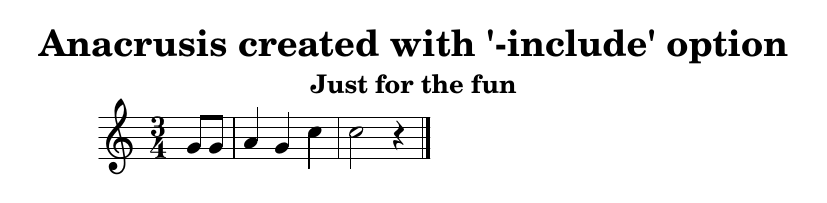
\includegraphics[scale=0.7]{../graphics/AnacrusisWithInclude.png}


% -------------------------------------------------------------------------
\section{Options values and arguments in included files}
% -------------------------------------------------------------------------

As shown in \sectionRef{Quoting, variables and aliases}, the shell identifies words in the command line. This is why options values and arguments have to be inclosed in \quotes\ or \doubleQuotes\ when they contain spaces.

In included files, these values are merely extracted from a line, and taken verbatim. To ease copying/pasting from the \CLI\, though, any \quotes\ or \doubleQuotes\ around the values are ignored.

For example, \mxmlfile{basic/QuotingInIncludedOptionsFiles.txt} contains:
\begin{lstlisting}[language=Terminal]
jacquesmenu@macmini: ~/musicformats-git-dev/files/musicxmlfiles/basic > cat QuotingInIncludedOptionsFiles.txt
# contents
  -title This year's title
  -subtitle 'Last year's quoted multi-word subtitle'
  -subsubtitle "Double quoted multi-word subsubtitle"

# display
  -display-options-values

# LilyPond
  -lilypond-generation-infos

# output
  -auto-output-file-name
\end{lstlisting}

Including this file and displaying the options values, we get:
\begin{lstlisting}[language=Terminal]
jacquesmenu@macmini: ~/musicformats-git-dev/files/musicxmlfiles/basic > xml2ly -include QuotingInIncludedOptionsFiles.txt HelloWorld.xml
  The options values for xml2ly are:
    Files group (-help-files-group, -hfiles-group), 1 atom chosen:
    --------------------------
      Files (-help-files, -hfiles), 1 atom chosen:
        fAutoOutputFileName                      : true

    Options and help group (-help-oah-group, -hoah-group), 1 atom chosen:
    --------------------------
      Options and help (-help-oah, -hoah), 1 atom chosen:
        fDisplayOptionsValues                    : true

    Header group (-help-header-group, -hheader-group), 3 atoms chosen:
    --------------------------
      Header (-help-header, -hheader), 3 atoms chosen:
        fTitle                                   : This year's title
        fSubTitle                                : Last year's quoted multi-word subtitle
        fSubSubTitle                             : Double quoted multi-word subsubtitle

    Output group (-help-output-group, -houtput-group), 1 atom chosen:
    --------------------------
      Output (-help-output, -houtput), 1 atom chosen:
        fXml2lyInfos                             : true
\end{lstlisting}


% -------------------------------------------------------------------------
\section{Multi-level includes}
% -------------------------------------------------------------------------

A file containing options and argument may itself use the \optionNameBoth{include}{inc} option, which allows for options to be shared easily for various uses of the services.

Note, however, that \earlyOption s are detected \MainIt{before} the files inclusion are performed. In particular, the \optionNameBoth{insider}{ins} option should be in the \CLI\ itself, at the top level so to say, to be taken into account.

For example, \mxmlfile{basic/HelloWorldOptionsAndArguments_1.txt} contains:
\begin{lstlisting}[language=Terminal]
jacquesmenu@macmini: ~/musicformats-git-dev/files/musicxmlfiles > cat basic/HelloWorldOptionsAndArguments_1.txt
# output file
 -auto-output-file-name

# contents
  -title 'My title'
  -subtitle "  Nice subtitle"
  -subsubtitle "Subsubtitle from HelloWorldOptionsAndArguments_1.txt"

# layout
  -global-staff-size 30

# non-musical
  -display-cpu-usage

# the MusicXML file
  basic/HelloWorld.xml

# nested include
  -include basic/HelloWorldOptionsAndArguments_2.txt
\end{lstlisting}

The included \mxmlfile{basic/HelloWorldOptionsAndArguments_2.txt} file contains:
\begin{lstlisting}[language=Terminal]
jacquesmenu@macmini: ~/musicformats-git-dev/files/musicxmlfiles > cat basic/HelloWorldOptionsAndArguments_2.txt
# non-musical
  -subsubtitle "Subsubtitle from HelloWorldOptionsAndArguments_2.txt"

# cycle detection check
#  -include HelloWorldOptionsAndArguments_1.txt
\end{lstlisting}

Including \mxmlfile{basic/HelloWorldOptionsAndArguments_1.txt}, we get:
\begin{lstlisting}[language=Terminal]
jacquesmenu@macmini: ~/musicformats-git-dev/files/musicxmlfiles > xml2ly -include basic/HelloWorldOptionsAndArguments_1.txt
Timing information:

Activity  Description                                             Kind       CPU (sec)
--------  ------------------------------------------------------  ---------  ---------

          Handle the options and arguments from argc/argv         mandatory    0.02962
Pass 1    Create an MXSR reading a MusicXML file                  mandatory    0.00362
Pass 2a   Create an MSR skeleton from the MXSR                    mandatory    0.00185
Pass 2b   Populate the MSR skeleton from MusicXML data            mandatory    0.00288
Pass 3    Convert the first MSR into a second MSR                 mandatory    0.00092
Pass 4    Convert the second MSR into an LPSR                     mandatory    0.00090
Pass 5    Convert the LPSR score to LilyPond code                 mandatory    0.00143

Total (sec)  Mandatory  Optional
-----------  ---------  ---------
0.04122      0.04122    0.00000
\end{lstlisting}

The resulting score is:\\
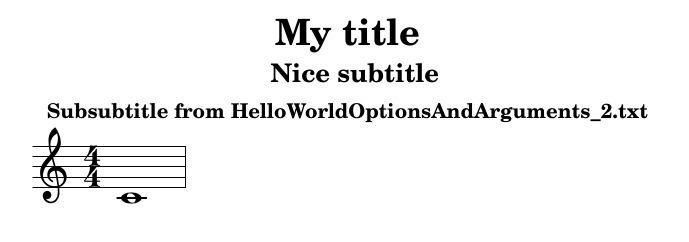
\includegraphics[scale=0.7]{../graphics/HelloWorldWithMultiLevelInclude.png}


% -------------------------------------------------------------------------
\section{Multi-level includes overflow}
% -------------------------------------------------------------------------

There are resources limitations on the machines \mf\ is used on, and we should prevent them to be overflown. This could occur is including a file runs into a loop in which the same file is included again.

\mf\ prevents this by limiting the level of such includes.

Let us uncomment the \optionName{include}{inc} option in \mxmlfile{basic/HelloWorldOptionsAndArguments_2.txt}, leading to:
\begin{lstlisting}[language=Terminal]
jacquesmenu@macmini: ~/musicformats-git-dev/files/musicxmlfiles > cat basic/HelloWorldOptionsAndArguments_2.txt
# non-musical
  -subsubtitle "Subsubtitle from HelloWorldOptionsAndArguments_2.txt"

# cycle detection check
  -include basic/HelloWorldOptionsAndArguments_1.txt
\end{lstlisting}

Now we get:
\begin{lstlisting}[language=Terminal]
jacquesmenu@macmini: ~/musicformats-git-dev/files/musicxmlfiles > xml2ly -include basic/HelloWorldOptionsAndArguments_1.txt
                        Including file [basic/HelloWorldOptionsAndArguments_1.txt]: more than 10 include levels, quitting
                        The include file names stack contains 10 elements:
                           1: [basic/HelloWorldOptionsAndArguments_2.txt]
                           2: [basic/HelloWorldOptionsAndArguments_1.txt]
                           3: [basic/HelloWorldOptionsAndArguments_2.txt]
                           4: [basic/HelloWorldOptionsAndArguments_1.txt]
                           5: [basic/HelloWorldOptionsAndArguments_2.txt]
                           6: [basic/HelloWorldOptionsAndArguments_1.txt]
                           7: [basic/HelloWorldOptionsAndArguments_2.txt]
                           8: [basic/HelloWorldOptionsAndArguments_1.txt]
                           9: [basic/HelloWorldOptionsAndArguments_2.txt]
                          10: [basic/HelloWorldOptionsAndArguments_1.txt]
\end{lstlisting}

